\documentclass{article}

\usepackage{style,xcolor}

% Sub-preambles
% https://github.com/MartinScharrer/standalone

% Encodings
\usepackage{amsmath,amssymb,gensymb,textcomp}

% Better tables
% Wide tables go to https://tex.stackexchange.com/q/332902
\usepackage{array,multicol,multirow,siunitx,tabularx}
\usepackage{tabularray}

% Better enum
\usepackage{enumitem}

% Graphics
\usepackage{caption,float}

% Allow setting >max< width of figure
% Remove if unneeded
\usepackage[export]{adjustbox} % 'export' allows adjustbox keys in \includegraphics
\usepackage{mwe}

% Custom commands
% Remove if unneeded
\newcommand*\mean[1]{\bar{#1}}

\ocorso
\oreporttype{}
\title{\textit{Ratatouille23}}
\reportlayout%

\numberwithin{equation}{section}
\numberwithin{figure}{section}

\begin{document}

\coverpage%

\section*{Gruppo INGSW2223\_N\_04}
\begin{center}
  \begin{tblr}{hlines = {0.9pt}, vlines = {0.9pt}, row{1} = {marroneApp!60}, colspec = {X[c]X[c]X[c]}, width = \textwidth}
        \textbf{No.} & \textbf{Nome e Cognome} & \textbf{Matricola} \\
        1            & Luigi Vessella          & N86003354\\
        2            & Matteo Marino           & N86003963\\
        3            & Biagio Speranza         & N86002964\\
  \end{tblr}
\end{center}

\newpage
\tableofcontents
\newpage
\section{Descrizione del progetto}
    {\large 
        Ratatouille23 è un sistema finalizzato al supporto alla gestione e all’operatività di attività di
        ristorazione. Il sistema consiste in un’applicazione performante e affidabile, attraverso cui gli utenti
        possono fruire delle funzionalità del sistema in modo intuitivo, rapido e piacevole. 
        La nostra visione della richiesta prevede lo sviluppo di un'applicazione mobile su sistema operativo Android che offrirà agli utilizzatori i seguenti servizi: 
    }
    
    \begin{itemize}
        \item \textit{ I proprietari (o amministratori) potranno creare account per i dipendenti}
        \item \textit{I proprietari saranno in grado di gestire uno o più ristoranti}
        \item \textit{Si avrà la possibilità di visualizzare e/o modificare il menu}
        \item \textit{I dipendenti (camerieri) saranno in grado di prendere e inoltrare le ordinazioni in cucina}
        \item \textit{Gli addetti alla cucina potranno avvisare i camerieri nel momento in cui è pronta un'ordinazione}
        \item \textit{Tutti potranno visionare lo storico delle ordinazioni con i dettagli}
    \end{itemize} 
    
    \begin{flushleft}
      {\large Ovviamente, il tipo di funzionalità messo a disposizione dall'applicativo sarà cambiato
        dinamicamente a seconda di chi si logga. 
        Gli amministratori e/o supervisori saranno inoltre dotati di tablet con a bordo l'OS di Google Android per
        una migliore fruizione della loro dashboard.}

      \vspace{1cm}

    {\large I dipendenti quali camerieri, operatori di cucina, capisala, saranno dotati di smartphone aziendali sempre con OS Android correttamente configurati per un'ottimale fruizione dell'applicazione.}
      \vspace{1cm}

    {\large \textbf{Tutti i dispositivi dovranno essere in grado di accedere a internet, preferibilmente per tutta la durata del servizio. Il funzionamento del server è invece garantito servizi allo stato dell'arte quali Microsoft Azure.}}
    \end{flushleft}
    
    \subsection{Premessa e presentazione}
    \begin{figure}[H]
        \centering
        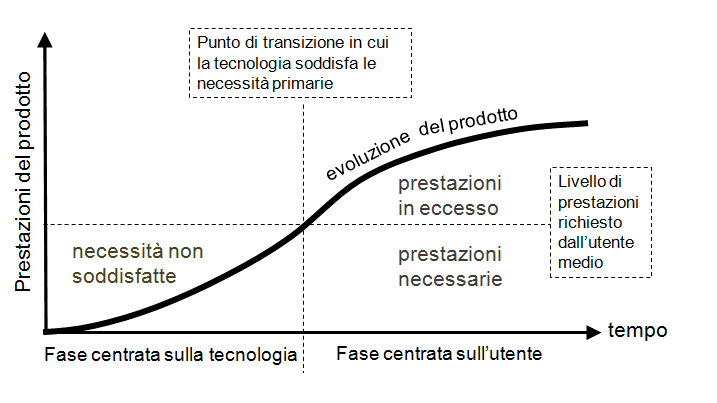
\includegraphics[scale=0.5]{assets/immagini varie/D.Norman grafico.png}
        \caption{\textbf{Grafico}: Evoluzione dei prodotti high-tech secondo D.Norman}\label{fig:Figure_D.Norman}
    \end{figure}

    \begin{flushleft}
        
        Con questo piccolo preambolo vogliamo richiamare l'attenzione sul diagramma di evoluzione dei prodotti software di D.Norman, il quale mostra il ciclo di vita che solitamente questo tipo di prodotto ha.
        All'inizio avremo un'app più incentrata sulle tecnologie implementate e/o da implementare per  "cercare " di raggiungere ciò che l'utente medio richiede dall'applicativo. Successivamente si otterrà il punto di pareggio in cui si soddisfano
        i bisogni dell'utente tipico, e ciò potrebbe essere considerato un buon punto di equilibrio del sistema.
        In fine, sempre ammesso che l'app sia sopravvissuta al mercato durante questo ciclo, ci può essere una fase finale con una condizione
        di iperfunzionalità, dove si cercherà via via di soddisfarre le esigenze di una platea di utenti più ampia. Nel caso della nostra applicazione Ratatouille23 descritta in questo documento, pensiamo di distribuire un prodotto nella sua 
        fase di equilibrio (vedere grafico) che certamente soddisfa le esigenze degli attori utilizzatori descritti nei punti successivi, ma che allo stesso tempo può essere facilmente aggiornata e migliorata qualora dovessero aggiungersi nuovi target d'utenti o cambiare
        gli esistenti.
    \end{flushleft}
 
    \section{Documento dei requisiti software}
    \subsection{Requisiti Funzionali}
        \begin{flushleft}  
            {\large
                Vengono qui presentati i requisiti funzionali dell'applicativo, ossia quei servizi che l'app  deve offrire agli utenti:
            } 
        \end{flushleft}
        
        \subsubsection{Admin}
        

        \begin{center}
          % Admin 1
          \begin{tblr}{hlines = {0.9pt}, vlines = {0.9pt}, row{1} = {marroneApp!60}, colspec = {X[c]X[l]}, width = \textwidth}
                  \textbf{ID}         & Admin\_1                             \\
                  \textbf{Nome}       & Registrazione account amministratore \\
                  \textbf{Descrizione} & {Il sistema permette ad un amministratore non registrato di registrarsi alla\\ piattaforma utilizzando: \textit{nome}, \textit{cognome}, \textit{email}, \textit{codice fiscale}, \textit{P.IVA} e \textit{password}}
          \end{tblr}

          \vspace{1cm}

          % Admin 2
          \begin{tblr}{hlines = {0.9pt}, vlines = {0.9pt}, row{1} = {marroneApp!60}, colspec = {X[c]X[l]}, width = \textwidth}
                  \textbf{ID}         & Admin\_2                             \\
                  \textbf{Nome}       & Modifica account amministratore \\
                  \textbf{Descrizione} & {Il sistema permette ad un amministratore loggato di modifcare i campi del proprio account}
          \end{tblr}

          \vspace{1cm}

          % Admin 3
          \begin{tblr}{hlines = {0.9pt}, vlines = {0.9pt}, row{1} = {marroneApp!60}, colspec = {X[c]X[l]}, width = \textwidth}
                  \textbf{ID}         & Admin\_3                             \\
                  \textbf{Nome}       & Registrazione dei dipendenti \\
                  \textbf{Descrizione} & {Il sistema permette ad un amministratore di creare utenze per i dipendenti non registrati del ristorante,\\ specificandone \textit{nome}, \textit{cognome}, \textit{email} e \textit{ruolo}}
          \end{tblr}

          \vspace{1cm}

          % Admin 4
          \begin{tblr}{hlines = {0.9pt}, vlines = {0.9pt}, row{1} = {marroneApp!60}, colspec = {X[c]X[l]}, width = \textwidth}
                  \textbf{ID}          & Admin\_4                             \\
                  \textbf{Nome}        & Modificare/Eliminare account dipendenti  \\
                  \textbf{Descrizione} & {Il sistema permette ad un amministratore loggato di modificare gli account dei propri dipendenti.}
          \end{tblr}

          \vspace{1cm}

          % Admin 5
          \begin{tblr}{hlines = {0.9pt}, vlines = {0.9pt}, row{1} = {marroneApp!60}, colspec = {X[c]X[l]}, width = \textwidth}
                  \textbf{ID}          & Admin\_5                             \\
                  \textbf{Nome}        & Aggiungere personale della cucina  \\
                  \textbf{Descrizione} & {Il sistema permette ad un amministratore loggato di aggiungere al proprio ristorante il personale della cucina.}
          \end{tblr}

          \vspace{1cm}

          % Admin 6
          \begin{tblr}{hlines = {0.9pt}, vlines = {0.9pt}, row{1} = {marroneApp!60}, colspec = {X[c]X[l]}, width = \textwidth}
                  \textbf{ID}          & Admin\_6                             \\
                  \textbf{Nome}        & Aggiunta dei Ristoranti  \\
                  \textbf{Descrizione} & {Il sistema permette ad un amministratore di poter aggiungere le proprie attività di ristorazione (CAMPI DA DEFINIRE).}
          \end{tblr}

          \vspace{1cm}

          % Admin 7
          \begin{tblr}{hlines = {0.9pt}, vlines = {0.9pt}, row{1} = {marroneApp!60}, colspec = {X[c]X[l]}, width = \textwidth}
                  \textbf{ID}          & Admin\_7                             \\
                  \textbf{Nome}        &  Modifica/Eliminazione dei Ristoranti  \\
                  \textbf{Descrizione} & {Il sistema permette ad un amministratore di poter modificare ed eliminare le proprie attività di ristorazione del sistema.}
          \end{tblr}

          \vspace{1cm}

          % Admin 8
          \begin{tblr}{hlines = {0.9pt}, vlines = {0.9pt}, row{1} = {marroneApp!60}, colspec = {X[c]X[l]}, width = \textwidth}
                  \textbf{ID}          & Admin\_8                             \\
                  \textbf{Nome}        &  Modifica dati dei Dipendenti  \\
                  \textbf{Descrizione} & {Il sistema permette ad un amministratore loggato di poter cambiare i dati personali dei dipendenti (nome, cognome, email, luogo).}
          \end{tblr}

          \vspace{1cm}

          % Admin 9
          \begin{tblr}{hlines = {0.9pt}, vlines = {0.9pt}, row{1} = {marroneApp!60}, colspec = {X[c]X[l]}, width = \textwidth}
                  \textbf{ID}          & Admin\_9                             \\
                  \textbf{Nome}        &  Aggiungere/Modificare elementi nel menù  \\
                  \textbf{Descrizione} & {Il sistema permette ad un amministratore o supervisore dell'attività di ristorazione di aggiungere/modificare elementi nel menù dell'attività. Ogni elemento dovrà avere i seguenti campi:\\ Nome, Costo, Descrizione, Elenco di Allergeni, Categoria/e}
          \end{tblr}

          \vspace{1cm}

          % Admin 10
          \begin{tblr}{hlines = {0.9pt}, vlines = {0.9pt}, row{1} = {marroneApp!60}, colspec = {X[c]X[l]}, width = \textwidth}
                  \textbf{ID}          & Admin\_10                             \\
                  \textbf{Nome}        &  Modifica dati personali\\
                  \textbf{Descrizione} & {Il sistema permette ad un amministratore loggato di poter cambiare i propri dati  personali.}
          \end{tblr}

          \vspace{1cm}

          % Admin 12
          \begin{tblr}{hlines = {0.9pt}, vlines = {0.9pt}, row{1} = {marroneApp!60}, colspec = {X[c]X[l]}, width = \textwidth}
                  \textbf{ID}          & Admin\_12                             \\
                  \textbf{Nome}        &  Tradurre il menu           \\
                  \textbf{Descrizione} & {Il sistema permette ad un Amministratore di poter tradurre gli elementi del proprio menù in un altra lingua}
          \end{tblr}

          \vspace{1cm}

          % Admin 13
          \begin{tblr}{hlines = {0.9pt}, vlines = {0.9pt}, row{1} = {marroneApp!60}, colspec = {X[c]X[l]}, width = \textwidth}
                  \textbf{ID}          & Admin\_13                             \\
                  \textbf{Nome}        &  Visualizza statistiche personale della cucina\\
                  \textbf{Descrizione} & {Il sistema permette ad un Amministratore di visualizzare, grazie anche all'ausilio di grafici interattivi, informazioni sull'operato degli addetti alla cucina}
          \end{tblr}

          \vspace{1cm}

          % Admin 14
          \begin{tblr}{hlines = {0.9pt}, vlines = {0.9pt}, row{1} = {marroneApp!60}, colspec = {X[c]X[l]}, width = \textwidth}
                  \textbf{ID}          & Admin\_14                             \\
                  \textbf{Nome}        & Modifica menu \\
                  \textbf{Descrizione} & {Il sistema permette ad un Amministratore di poter aggiornare (aggiungere, modificare ed eliminare elementi) il menu del ristorante}
          \end{tblr}
        \end{center}

        \subsubsection{Cameriere}
        \begin{center}

          % Waiter 1
          \begin{tblr}{hlines = {0.9pt}, vlines = {0.9pt}, row{1} = {marroneApp!60}, colspec = {X[c]X[l]}, width = \textwidth}
                  \textbf{ID}          & Waiter\_1                             \\
                  \textbf{Nome}        & Prendere le ordinazioni \\
                  \textbf{Descrizione} & {Il sistema permette ai camerieri di prendere ordinazioni ai tavoli, inoltrandole alla cucina.}
          \end{tblr}

          \vspace{1cm}

          % Waiter 2
          \begin{tblr}{hlines = {0.9pt}, vlines = {0.9pt}, row{1} = {marroneApp!60}, colspec = {X[c]X[l]}, width = \textwidth}
                  \textbf{ID}          & Waiter\_2                             \\
                  \textbf{Nome}        & Gestione delle ordinazioni \\
                  \textbf{Descrizione} & {Il sistema permette ai camerieri di prendere ordinazioni ai tavoli, inoltrandole alla cucina.}
          \end{tblr}

          \vspace{1cm}

          % Waiter 3
          \begin{tblr}{hlines = {0.9pt}, vlines = {0.9pt}, row{1} = {marroneApp!60}, colspec = {X[c]X[l]}, width = \textwidth}
                  \textbf{ID}          & Waiter\_3                             \\
                  \textbf{Nome}        & Evasione degli ordini \\
                  \textbf{Descrizione} & {Il sistema permette a un Cameriere di marcare i singoli elementi di un ordine come conclusi, aggiornando gli addetti in cucina}
          \end{tblr}

          \vspace{1cm}

          % Waiter 4
          \begin{tblr}{hlines = {0.9pt}, vlines = {0.9pt}, row{1} = {marroneApp!60}, colspec = {X[c]X[l]}, width = \textwidth}
                  \textbf{ID}          & Waiter\_4                             \\
                  \textbf{Nome}        & Sollecitare la cucina \\
                  \textbf{Descrizione} & {Il sistema permette a un Cameriere di sollecitare la cucina nel caso in cui un ordine sia da troppo tempo in preparazione }
          \end{tblr}

        \end{center}
        
        \subsubsection{Cucina}

        \begin{center}
          % Kitchen 1
          \begin{tblr}{hlines = {0.9pt}, vlines = {0.9pt}, row{1} = {marroneApp!60}, colspec = {X[c]X[l]}, width = \textwidth}
                  \textbf{ID}          & Kitchen\_1                             \\
                  \textbf{Nome}        & Marcare gli ordini pronti \\
                  \textbf{Descrizione} & {Il sistema permette alla cucina di marcare gli ordini pronti alla "consegna", specificando lo chef che l'ha preparato}
          \end{tblr}

          \vspace{1cm}

          % Kitchen 2
          \begin{tblr}{hlines = {0.9pt}, vlines = {0.9pt}, row{1} = {marroneApp!60}, colspec = {X[c]X[l]}, width = \textwidth}
                  \textbf{ID}          & Kitchen\_2                             \\
                  \textbf{Nome}        & Sollecitare i camerieri \\
                  \textbf{Descrizione} & {Il sistema permette alla cucina di notificare i camerieri nel caso in cui un ordine sia pronto alla consegna da troppo tempo }
          \end{tblr}

        \end{center}

        \subsubsection{Supervisore}

        \begin{center}

          % Hypervisor 1 (Forse Supervisor (?))
          \begin{tblr}{hlines = {0.9pt}, vlines = {0.9pt}, row{1} = {marroneApp!60}, colspec = {X[c]X[l]}, width = \textwidth}
                  \textbf{ID}          & Hypervisor\_1                             \\
                  \textbf{Nome}        & Avvisare il personale \\
                  \textbf{Descrizione} & {Il sistema permette ad un supervisore ed un amministratore di inviare degli avvisi al personale}
          \end{tblr}

          \vspace{1cm}

          % Hypervisor 2 (Forse Supervisor (?))
          \begin{tblr}{hlines = {0.9pt}, vlines = {0.9pt}, row{1} = {marroneApp!60}, colspec = {X[c]X[l]}, width = \textwidth}
                  \textbf{ID}          & Hypervisor\_2                             \\
                  \textbf{Nome}        & Visualizzare stato ordini per tavolo\\
                  \textbf{Descrizione} & {Il sistema permette ad un Supervisore ed un Cameriere di visualizzare gli stati delle ordinazioni per ogni tavolo}
          \end{tblr}

          \vspace{1cm}

          % Hypervisor 3 (Forse Supervisor (?))
          \begin{tblr}{hlines = {0.9pt}, vlines = {0.9pt}, row{1} = {marroneApp!60}, colspec = {X[c]X[l]}, width = \textwidth}
                  \textbf{ID}          & Hypervisor\_3                             \\
                  \textbf{Nome}        & Visualizzare ordini in arrivo\\
                  \textbf{Descrizione} & {Il sistema permette ad un Supervisore e alla Cucina di visualizzare l'elenco di ordini in arrivo}
          \end{tblr}

          \vspace{1cm}

          % Hypervisor 4 (Forse Supervisor (?))
          \begin{tblr}{hlines = {0.9pt}, vlines = {0.9pt}, row{1} = {marroneApp!60}, colspec = {X[c]X[l]}, width = \textwidth}
                  \textbf{ID}          & Hypervisor\_4                             \\
                  \textbf{Nome}        & Visualizzare ordini in uscita\\
                  \textbf{Descrizione} & {Il sistema permette ad un Supervisore e alla Cucina di visualizzare l'elenco di ordini pronti all'uscita}
          \end{tblr}

          \vspace{1cm}

          % Hypervisor 5 (Forse Supervisor (?))
          \begin{tblr}{hlines = {0.9pt}, vlines = {0.9pt}, row{1} = {marroneApp!60}, colspec = {X[c]X[l]}, width = \textwidth}
                  \textbf{ID}          & Hypervisor\_5                             \\
                  \textbf{Nome}        & Visualizzare storico ordini\\
                  \textbf{Descrizione} & {Il sistema permette ad un Supervisore e alla Cucina di visualizzare lo storico degli ordini}
          \end{tblr}

          \vspace{1cm}
        \end{center}


        \subsubsection{Tutti}

        \begin{center}

          % All 1
          \begin{tblr}{hlines = {0.9pt}, vlines = {0.9pt}, row{1} = {marroneApp!60}, colspec = {X[c]X[l]}, width = \textwidth}
                  \textbf{ID}          & All\_1                             \\
                  \textbf{Nome}        & Recupero/Cambio Password\\
                  \textbf{Descrizione} & {Il sistema permette a tutti gli utenti registrati di poter recuperare la password e di poterla modificare}
          \end{tblr}

          \vspace{1cm}

          % All 2
          \begin{tblr}{hlines = {0.9pt}, vlines = {0.9pt}, row{1} = {marroneApp!60}, colspec = {X[c]X[l]}, width = \textwidth}
                  \textbf{ID}          & All\_2                             \\
                  \textbf{Nome}        & Login\\
                  \textbf{Descrizione} & {Il sistema permette a tutti gli utenti registrati di poter effettuare il login con Username e Password all'interno della piattaforma}
          \end{tblr}

          \vspace{1cm}

          % All 3
          \begin{tblr}{hlines = {0.9pt}, vlines = {0.9pt}, row{1} = {marroneApp!60}, colspec = {X[c]X[l]}, width = \textwidth}
                  \textbf{ID}          & All\_3                             \\
                  \textbf{Nome}        & Visualizzare un avviso o sollecitazione\\
                  \textbf{Descrizione} & {Il sistema permette a tutti gli utenti registrati pi poter visualizzare gli avvisi e le sollecitazioni ricevuti, marcandoli come visualizzati}
          \end{tblr}
        \end{center}

        \newpage

        \subsection{Requisiti Non Funzionali}
        \begin{flushleft} Vengono qui elencati i requisiti non funzionali dell'applicativo: \end{flushleft}

        \begin{center}
          % Unfunctional 1
          \begin{tblr}{hlines = {0.9pt}, vlines = {0.9pt}, row{1} = {marroneApp!60}, colspec = {X[c]X[l]}, width = \textwidth}
                  \textbf{ID}          & Unfunctional\_1                             \\
                  \textbf{Nome}        & Policy first password\\
                  \textbf{Descrizione} & {Il sistema richiede al primo accesso di un dipendente il cambio della password provvisoria in una password personale.}
          \end{tblr}

          \vspace{1cm}

          % Unfunctional 2
          \begin{tblr}{hlines = {0.9pt}, vlines = {0.9pt}, row{1} = {marroneApp!60}, colspec = {X[c]X[l]}, width = \textwidth}
                  \textbf{ID}          & Unfunctional\_2                             \\
                  \textbf{Nome}        & Verifica esistenza della mail\\
                  \textbf{Descrizione} & {Al fine di evitare registrazioni con e-mail fittizie, il sistema richiede l'autenticazione della mail mediante codice di verifica per poter procedere con il completamento della registrazione}
          \end{tblr}

          \vspace{1cm}

          % Unfunctional 3
          \begin{tblr}{hlines = {0.9pt}, vlines = {0.9pt}, row{1} = {marroneApp!60}, colspec = {X[c]X[l]}, width = \textwidth}
                  \textbf{ID}          & Unfunctional\_3                             \\
                  \textbf{Nome}        & Password Strength\\
                  \textbf{Descrizione} & {Al fine di evitare la creazione di password poco sicure, il sistema impone all'utente di utilizzare una password di almeno 8 caratteri che contenga numeri e caratteri speciali.}
          \end{tblr}

          \vspace{1cm}

          % Unfunctional 4
          \begin{tblr}{hlines = {0.9pt}, vlines = {0.9pt}, row{1} = {marroneApp!60}, colspec = {X[c]X[l]}, width = \textwidth}
                  \textbf{ID}          & Unfunctional\_4                             \\
                  \textbf{Nome}        & \textcolor{red}{TODO}\\
                  \textbf{Descrizione} & {Una P.IVA appartiene ad un solo amministratore.}
          \end{tblr}
        \end{center}

        \subsection{Requisiti di Dominio}

        \begin{center}
          % Domain 1
          \begin{tblr}{hlines = {0.9pt}, vlines = {0.9pt}, row{1} = {marroneApp!60}, colspec = {X[c]X[l]}, width = \textwidth}
                  \textbf{ID}          & Domain\_1                             \\
                  \textbf{Nome}        & GDPR\\
                  \textbf{Descrizione} & {Il sistema deve essere conforme alla normativa GDPR (Regolamento Generale  sulla Protezione dei Dati), per il trattamento dei dati personali e riguardante la privacy dell'utente}
          \end{tblr}
        \end{center}
    \subsection{Modellazione dei casi d'uso}

    \begin{flushleft}
        In questa sezione vengono riportati i Use-case diagram relativi al sistema, le tabelle di Cockburn e i Sequence diagram relativi alle funzionalità  \emph{\textbf{Aggiungi ristorante}},  \emph{\textbf{Aggiungi piatto}},  \emph{\textbf{Prendi ordinazione}},  \emph{\textbf{Visualizza avvisi}}.
    \end{flushleft}

    \subsubsection{Use-Case Diagram}
        \begin{flushleft}
            Qui viene riportato lo Use Case Diagram relativo all'applicazione, che per rendere la lettura più semplificata 
            è stato diviso in più sezioni.
        \end{flushleft}
        
        \begin{figure}[H]
            \centering
            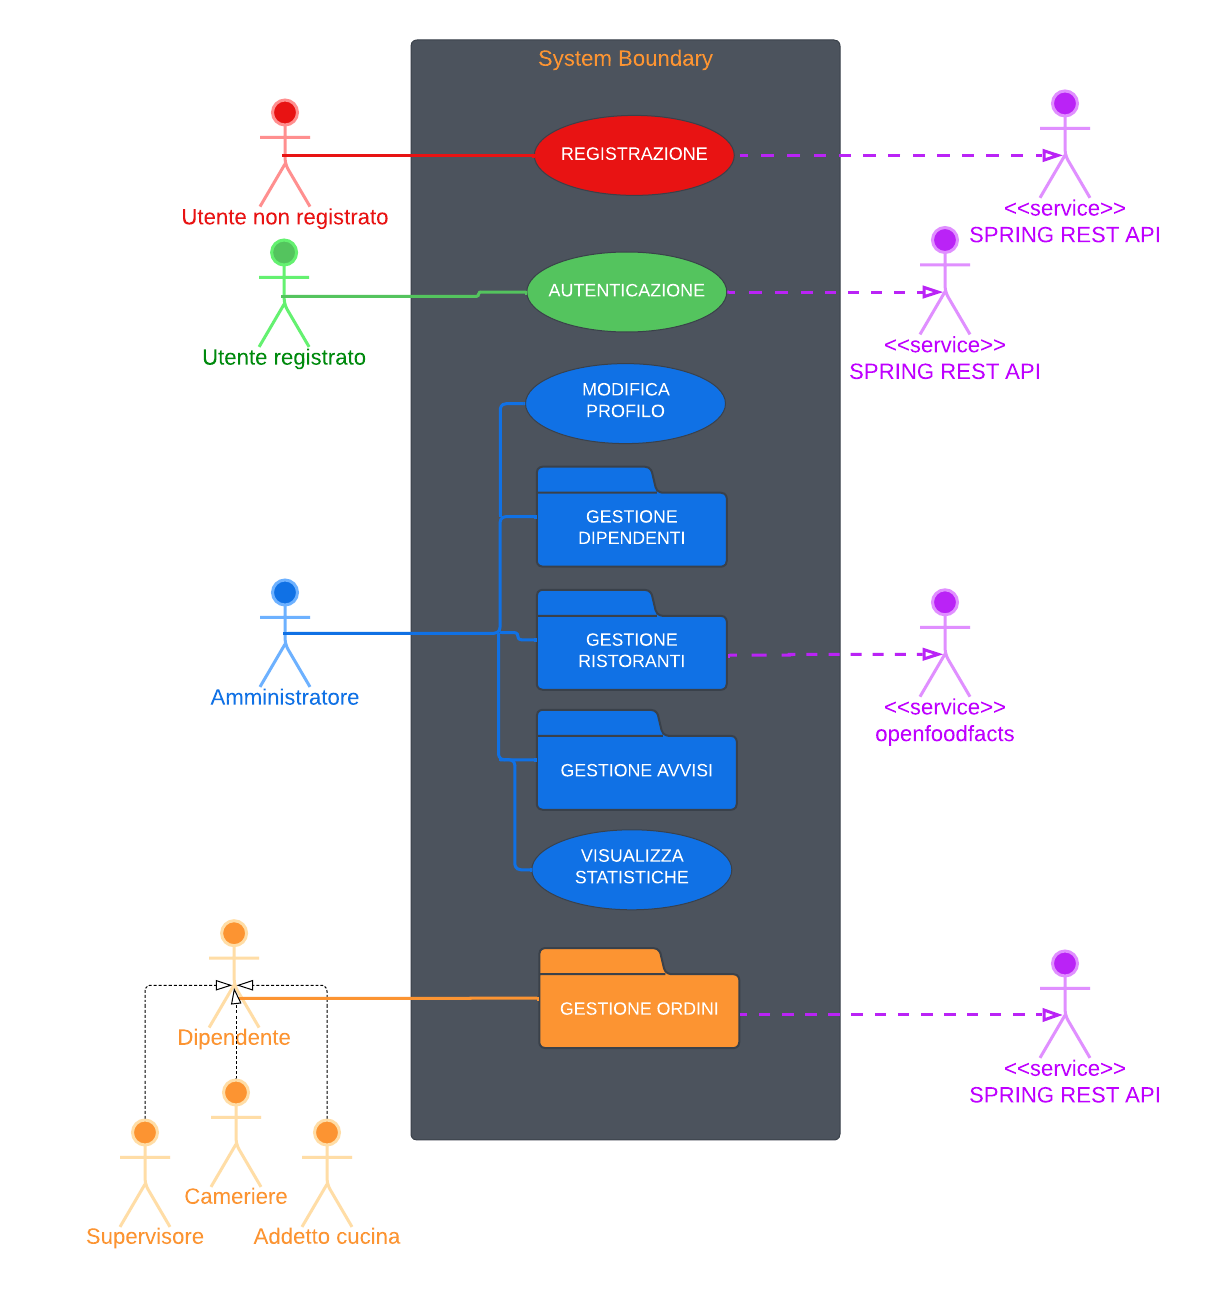
\includegraphics[width=0.8\textwidth]{assets/diagrammi/Use-Case/Use-Case Generale.png}
            \caption{Use Case dell'applicazione}
            \label{fig:ucdGenerale}
        \end{figure}
        
        \begin{figure}[H]
            \centering
            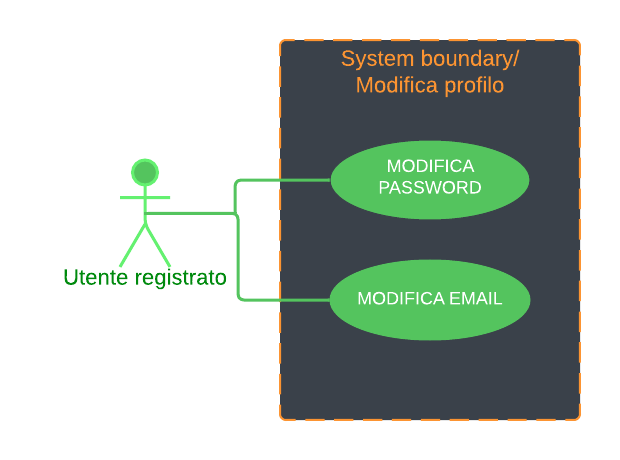
\includegraphics[width=0.8\textwidth]{assets/diagrammi/Use-Case/Modifica Profilo.png}
            \caption{Use Case relativo alla modifica del profilo}
            \label{fig:ucdModProfile}
        \end{figure}

        \begin{figure}[H]
            \centering
            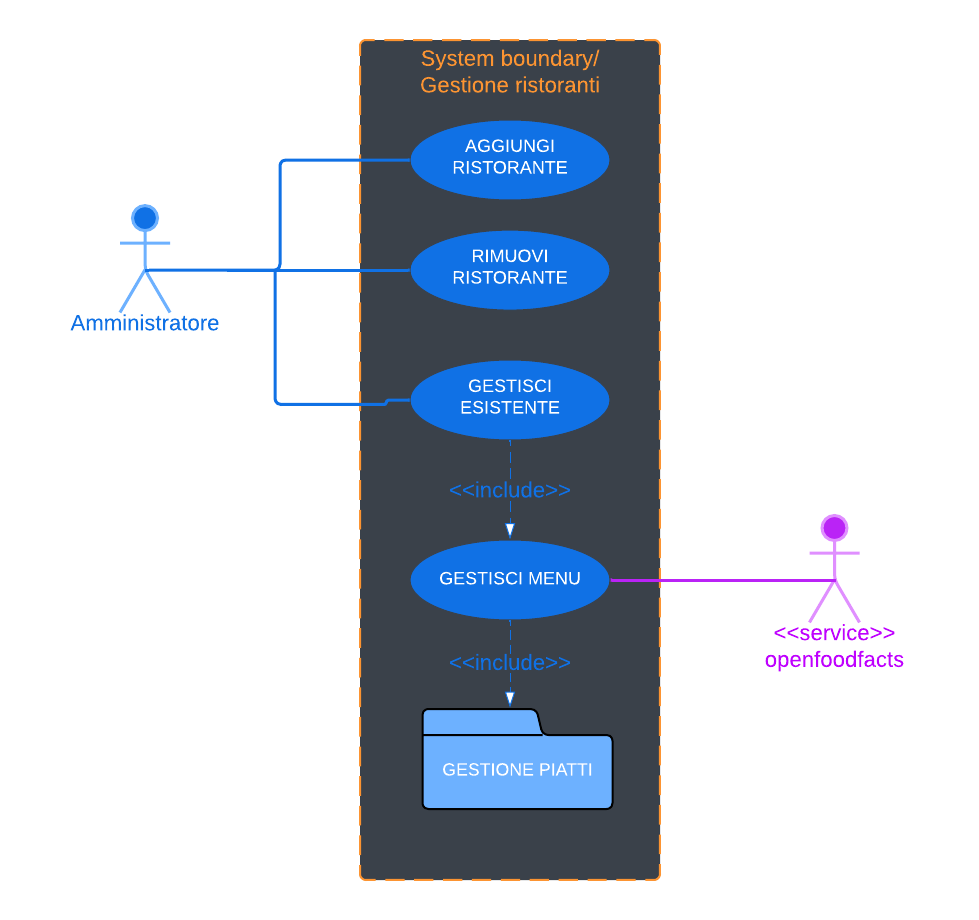
\includegraphics[width=0.8\textwidth]{assets/diagrammi/Use-Case/Gestione ristoranti.png}
            \caption{Use Case relativo alla gestione dei ristoranti}
            \label{fig:ucdResturantMgmt}
        \end{figure}

        \begin{figure}[H]
            \centering
            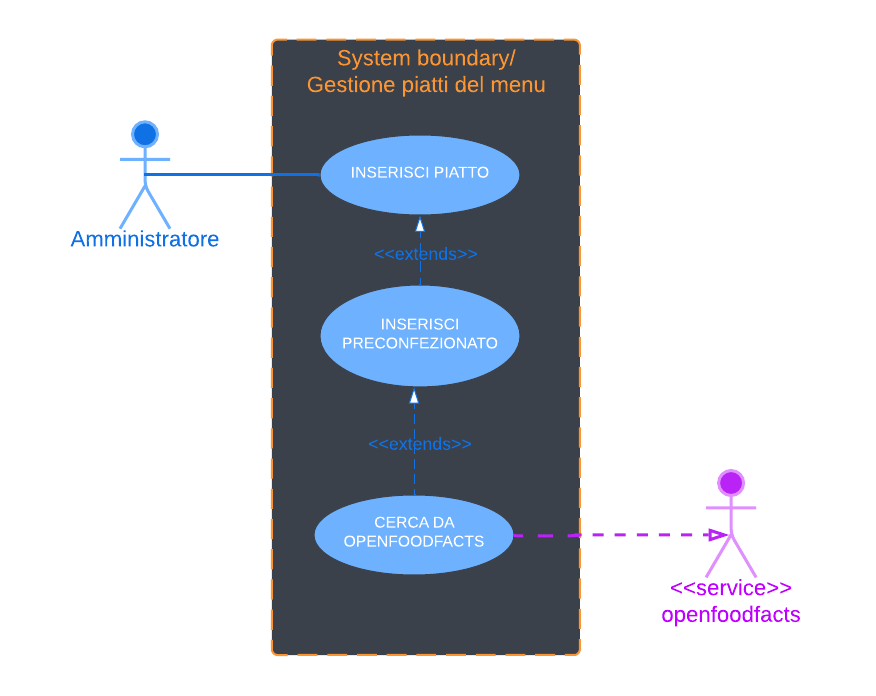
\includegraphics[width=0.8\textwidth]{assets/diagrammi/Use-Case/Gestione piatti.png}
            \caption{Use Case relativo alla gestione dei piatti del menù}
            \label{fig:ucdPlatesMgmt}
        \end{figure}

        \begin{figure}[H]
            \centering
            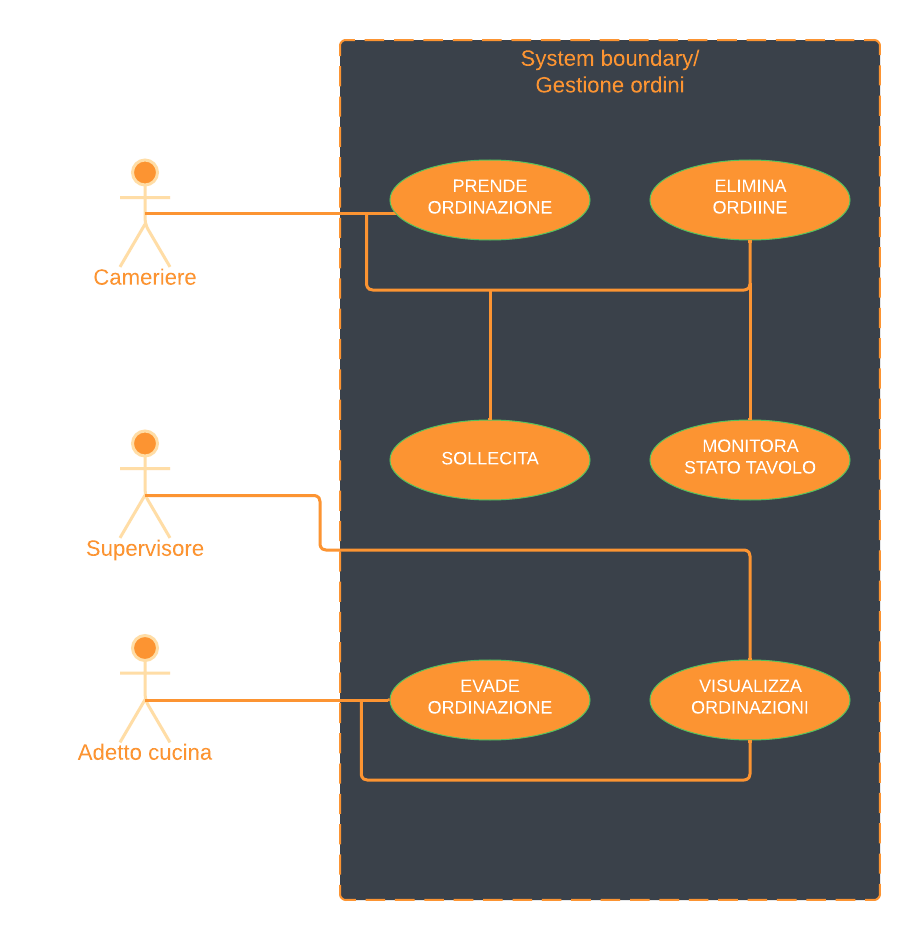
\includegraphics[width=0.7\textwidth]{assets/diagrammi/Use-Case/Gestione ordini.png}
            \caption{Use Case relativo alla gestione degli ordini}
            \label{fig:ucdOrderMgmt}
        \end{figure}
        
        \begin{figure}[H]
            \centering
            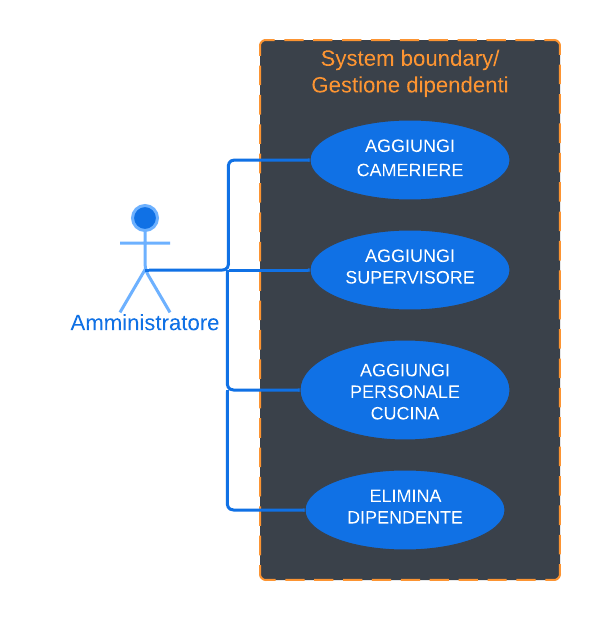
\includegraphics[width=0.6\textwidth]{assets/diagrammi/Use-Case/Gestione dipendenti.png}
            \caption{Use Case relativo alla gestione dei dipendenti}
            \label{fig:ucdWorkersMgmt}
        \end{figure}

        \begin{figure}[H]
            \centering
            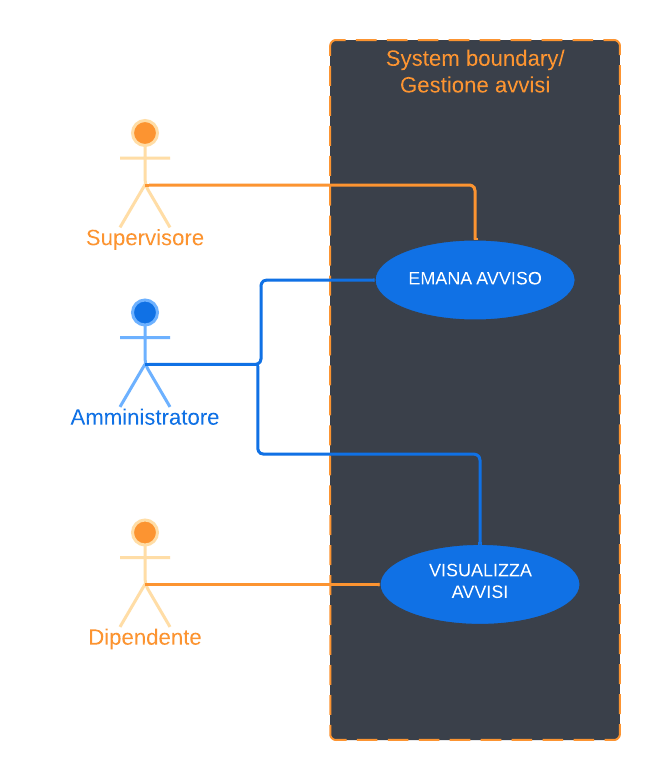
\includegraphics[width=0.8\textwidth]{assets/diagrammi/Use-Case/Gestione avvisi.png}
            \caption{Use Case relativo alla gestione degli avvisi}
            \label{fig:ucdAdvMgmt}
        \end{figure}
\newpage
    \subsubsection{Tabelle di Cockburn} %sezione 2.7
    \begin{flushleft}
        Vengono qui riportate le tabelle di cockburn dei casi d'uso \textit{\textbf{Aggiungi ristorante}}, \textit{\textbf{Aggiungi piatto}}, \textit{\textbf{Prendi ordinazione}}, \textit{\textbf{Visualizza avvisi}}.
    \end{flushleft}

    \begin{center}
      \begin{longtblr}{hlines = {0.9pt}, vlines = {0.9pt}, row{1}={marroneApp!60},colspec = {X[c]X[c]X[c]X[c]}, width = \textwidth,  rowhead=1}
        \textbf{Use Case \#1} & \SetCell[c=3]{c} \textbf{Aggiunta ristorante} \\
        \textbf{Goal in Context} & \SetCell[c=3]{l}{Un admin (proprietario di uno o più ristoranti)\\ vuole aggiungere uno di questi nell' app Ratatuille.}\\

        \textbf{Precodition} & \SetCell[c=3]{l}{Il proprietario deve essere registrato e loggato nell'app come amministratore}\\

        \textbf{Success End Condition} & \SetCell[c=3]{l}{Il proprietario aggiunge correttamente il ristorante}\\

        \textbf{Failed End Condition}  & \SetCell[c=3]{l}{Il proprietario non riesce ad aggiungere il ristorante}\\

        \textbf{Primary Actor}  & \SetCell[c=3]{c}{Amministratore}\\
        \textbf{Trigger}  & \SetCell[c=3]{c}{Preme il pulsante "Aggiungi"}\\

        \SetCell[r=5]{c}\textbf{Description}  & Step & UserAction & System\\
                                              & 1    & {L'amministratore preme sul tasto \textit{"AGGIUNGI RISTORANTE"}\\ sulla schermata \textbf{\textit{M04}}} & \\
                                              & 2    &       & {Mostra la schermata \textbf{\textit{M06}}}\\
                                              & 3    &  {Compila i campi necessari per la registrazione del proprio ristorante e preme sul tasto "SALVA" per aggiungere il Ristorante}     & \\
                                              & 4    &       & {Ricarica la schermata \textbf{\textit{M04}} aggiungendo nella lista dei ristoranti l'ultimo appena inserito} \\
        %% Extensions
        \SetCell[r=2]{c}{\textbf{Extension \#\ 1}\\ L'amministratore non fa nulla e torna indietro} & Step & UserAction & System\\
                                                                                                    & 4a   &  & Torna alla schermata \textbf{\textit{M04}}\\

        \SetCell[r=2]{c}{\textbf{Extension \#2}\\ L'amministratore ha aggiunto un ristorante già presenta nella propria lista di ristoranti} & Step & UserAction & System\\*
                                                  & 4b   &  & {Mostra uno dei messaggi di errore della schermata \textbf{\textit{{M0boh:}}} restando allo step \textbf{2} dello scenario principale}\\

        \SetCell[r=2]{c}{\textbf{Extension \#3}\\ L'amministratore ha lasciato uno o più campi vuoti}
                                                  & Step & UserAction & System\\
                                                  & 4c   &  & {Mostra uno o più dei messaggi di errore della schermata \textbf{\textit{{M0boh}}} restando allo step \textbf{2} dello scenario principale}\\

        \SetCell[r=2]{c}{\textbf{Extension \#4}\\ L'amministratore ha aggiunto un nome troppo corto}
                                                  & Step & UserAction & System\\
                                                  & 4d   &  & {Mostra il messaggio di errore di fianco al campo "Nome" della schermata \textbf{\textit{{M0boh}}} restando allo step \textbf{2} dello scenario principale} \\

        \SetCell[r=2]{c}{\textbf{Extension \#5}\\ L'amministratore ha aggiunto un numero di coperti non valido}
                                                  & Step & UserAction & System\\
                                                  & 4e   &  & {Mostra il messaggio di errore di fianco al campo "Numero di coperti" della schermata \textbf{\textit{{M0boh}}} restando allo step \textbf{2} dello scenario principale} \\

        \SetCell[r=2]{c}{\textbf{Extension \#6}\\ L'amministratore ha aggiunto un indirizzo troppo corto}
                                                  & Step & UserAction & System\\
                                                  & 4f   &  & {Mostra il messaggio di errore di fianco al campo "Indirizzo" della schermata \textbf{\textit{{M0boh}}} restando allo step \textbf{2} dello scenario principale} \\

        \SetCell[r=2]{c}{\textbf{Extension \#7}\\ L'amministratore ha aggiunto un numero di telefono non valido} 
                                                  & Step & UserAction & System\\*
                                                  & 4g   &  & {Mostra il messaggio di errore di fianco al campo "Numero di telefono" della schermata \textbf{\textit{{M0boh}}} restando allo step \textbf{2} dello scenario principale} \\

        %%% Subvariations
        \SetCell[r=4]{c}{\textbf{Subvariation \#1} \\ L' amministratore torna indietro completando solo parzialmente i campi}  & Step & UserAction & System\\
                                                                                                                             & 1 & & Mostra la schermata \textbf{\textit{M0boh}}\\
                                                                                                                             & 2 & {Preme su "SI"} & \\
                                                                                                                             & 3 & & Torna alla schermata \textbf{\textit{M04}}\\

        \SetCell[r=4]{c}{\textbf{Subvariation \#2} \\ L' amministratore inizialmente vuole tornare indietro completando solo parzialmente i campi ma cambia idea}
                                                        & Step & UserAction & System\\
                                                        & 1 & & Mostra la schermata \textbf{\textit{M0boh}}\\
                                                        & 2 & {Preme su "NO"} & \\
                                                        & 3 & & Torna alla schermata \textbf{\textit{M06}} alo step \textbf{2} dello scenario principale\\

        %\textbf{Notes}  & \SetCell[c=3]{c}{\textcolor{red}{TODO}}\\
      \end{longtblr}
    \end{center}

    \newpage
        
    \begin{center}
          \begin{longtblr}{hlines = {0.9pt}, vlines = {0.9pt}, row{1}={marroneApp!60}, colspec = {X[c]X[c]X[c]X[c]}, width = \textwidth}
            \textbf{Use Case \#2} & \SetCell[c=3]{c} \textbf{Aggiunta piatto al menù} \\
            \textbf{Goal in Context} & \SetCell[c=3]{l}{Un admin (proprietario di uno o più ristoranti) vuole aggiungere un piatto \\in un menu di un suo ristorante}\\
          
            \textbf{Precodition} & \SetCell[c=3]{l}{Il proprietario deve essere registrato e loggato nell'app come amministratore, \\deve aver aggiunto almeno un ristorane e deve averne creato un menu}\\
          
            \textbf{Success End Condition} & \SetCell[c=3]{l}{Il proprietario aggiunte correttamente un piatto al suo menu}\\
          
            \textbf{Failed End Condition}  & \SetCell[c=3]{l}{Il proprietario non riesce ad aggiungere un piatto al suo ristorante}\\
          
            \textbf{Primary Actor}  & \SetCell[c=3]{c}{Amministratore}\\
            \textbf{Trigger}  & \SetCell[c=3]{c}{Preme il pulsante "Accetta"}\\
            
            \SetCell[r=4]{c}\textbf{Description}  & Step & UserAction & System\\
                                          & 1 & {L'amministratore preme sul tasto \textit{"AGGIUNGI RISTORANTE"}\\ sulla schermata \textbf{\textit{M04}}} & \\
                                          & 2 &  TODO & System\\
                                          & 3 &       & TODO\\
          
            \SetCell[r=2]{c}\textbf{Extension}  & Step & UserAction & System\\
                                                & Step & UserAction & System\\
          
            \SetCell[r=2]{c}\textbf{Subvariation}  & Step & UserAction & System\\
                                                  & Step & UserAction & System\\
          
            %\textbf{Notes}  & \SetCell[c=3]{c}{\textcolor{red}{TODO}}\\
          \end{longtblr}
      \end{center}

    \subsection{Mock-up dell'applicazione}
    \begin{flushleft}
        Qui vengono presentati i mockup relativi all'applicazione.
    \end{flushleft}
    \subsubsection{Homepage dell'applicazione}
        \begin{figure}[H]
          \centering
          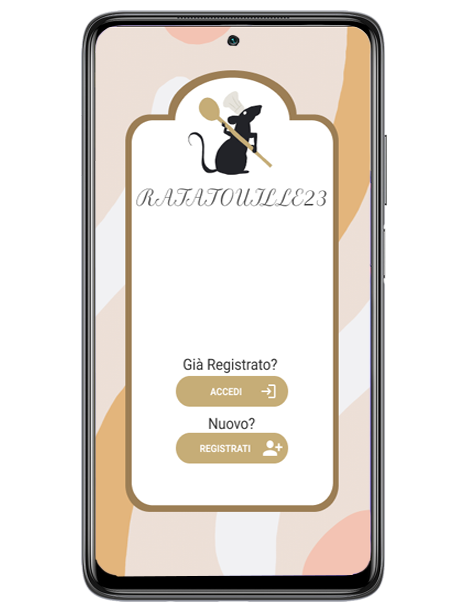
\includegraphics[scale=0.5]{assets/Mockup/Mockup_Homepage.png}
          \caption{\textbf{M01}: Homepage dell'applicazione}\label{fig:Mockup_Homepage}
        \end{figure}
        \begin{flushleft}
            \textbf{ID} \ \Large{\textit{\textbf{M01}}}\\
        \end{flushleft}

        \textbf{Componenti}:

        \begin{center}
          \begin{tblr}{hlines = {0.9pt}, vlines = {0.9pt}, row{1} = {marroneApp!60}, colspec = {X[c]X[c]X[c]}, width = \textwidth}
            \textbf{Tipo}  &   \textbf{Nome} & \textbf{Funzione} \\
            Bottone        &   ACCEDI        & Quando cliccato porta alla schermata \textit{\textbf{M02}} \\
            Bottone        &   REGISTRATI   & Quando cliccato porta alla schermata \textit{\textbf{M03}}  \\
          \end{tblr}
        \end{center}
        
        \newpage

        \subsubsection{Schermata di accesso nel sistema}
            \begin{figure}[H]
                \centering
                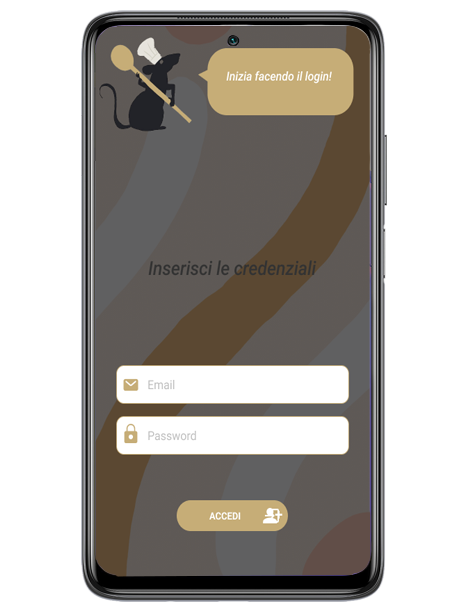
\includegraphics[scale=0.5]{assets/Mockup/Mockup_Accesso.png}
                \caption{\textbf{M02}: Schermata di accesso nel sistema}\label{fig:Mockup_Login}
            \end{figure}
            \begin{flushleft}
                \textbf{ID} \ \Large{\textit{\textbf{M02}}}\\
            \end{flushleft}

            \textbf{Componenti}:

            \begin{center}
              \begin{tblr}{hlines = {0.9pt}, vlines = {0.9pt}, row{1} = {marroneApp!60}, colspec = {X[c]X[c]X[c]}, width = \textwidth}
                \textbf{Tipo}   &   \textbf{Nome}   &   \textbf{Funzione} \\
                Edit Text       &   EMAIL &   Permette l'inserimento dell'email dell'utente \\
                Edit Text       &   PASSWORD  &  Permette l'inserimento della password dell'utente  \\
                Bottone         &   ENTRA   & Quando cliccato porta alla schermata \textit{\textbf{M04}} se admin, \textit{\textbf{M09}} se supervisore, \textit{\textbf{M11}} se cameriere,   \\
              \end{tblr}
            \end{center}

        \newpage
        \subsubsection{Schermata di registrazione nel sistema}
        \begin{figure}[H]
          \centering
          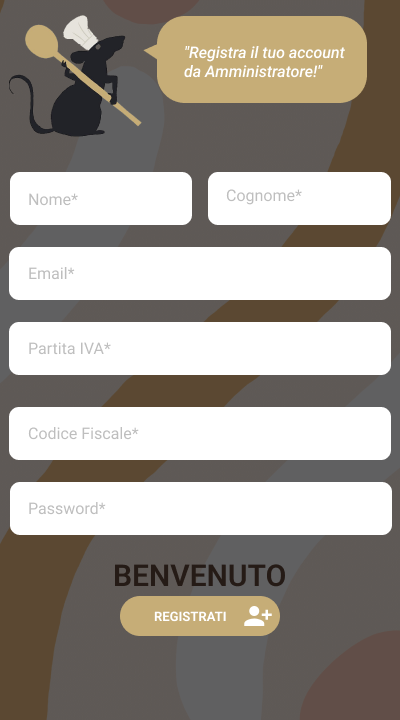
\includegraphics[scale=0.25]{assets/Mockup/Mockup_Register.png}
          \caption{\textbf{M03}: Schermata di registrazione nel sistema}\label{fig:Mockup_Register}
        \end{figure}

        \begin{flushleft}
          \textbf{ID} \ \Large{\textit{\textbf{M03}}}\\
          \large{\textit{Nota}: la schermata di registrazione è valida solo per gli admin proprietari dei ristoranti, in quanto sono poi loro a registrare i dipendenti.}\\
        \end{flushleft}

        \textbf{Componenti}:

            \begin{center}
              \begin{longtblr}{hlines = {0.9pt}, vlines = {0.9pt}, row{1} = {marroneApp!60}, colspec = {X[c]X[c]X[c]}, width = \textwidth, rowhead=1}
                \textbf{Tipo}   &   \textbf{Nome}   &   \textbf{Funzione} \\
                Edit Text    &   NOME    &   Permette di inserire il nome dell'admin \\
                Edit Text & COGNOME   &  Permette di inserire il cognome dell'admin \\
                Edit Text    &   PASSWORD    &   Permette di inserire una password per l'admin \\
                Edit Text    &   EMAIL   &   Permette di inserire l'email dell'admin \\
                Edit Text    & CODICE FISCALE    & Permette di inserire il codice fiscale dell'admin \\
                Edit Text    &   P.IVA   & Permette di inserire la partita IVA dell'admin \\
                Bottone &   REGISTRATI  & Quando cliccato riporta alla schermata \textit{\textbf{M01}} per permettere l'accesso \\
              \end{longtblr}
            \end{center}
        \newpage
        \subsubsection{Schermata home per gli admin}
        \begin{figure}[H]
            \centering
            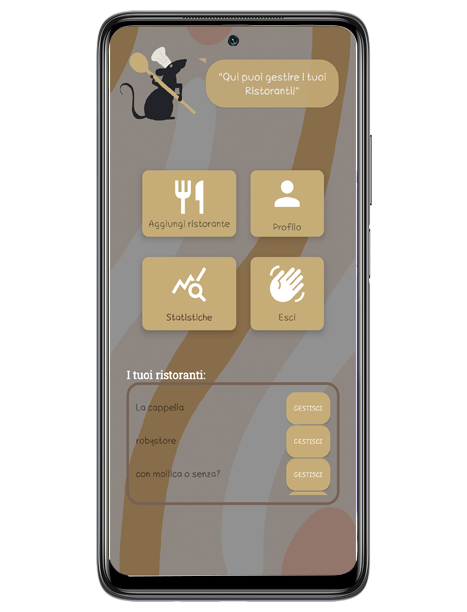
\includegraphics[scale=0.35]{assets/Mockup/Mockup_AdminDash.png}
            \caption{\textbf{M04}: Schermata home per gli admin}\label{fig:Mockup_AdminDashboard}
        \end{figure}
        \begin{flushleft}
            \textbf{ID} \ \Large{\textit{\textbf{M04}}} \\
        \end{flushleft}
        \textbf{Componenti}:

            \begin{center}
                \begin{longtblr}{hlines = {0.9pt}, vlines = {0.9pt}, row{1} = {marroneApp!60}, colspec = {X[c]X[c]X[c]}, width = \textwidth, rowhead=1}
                \textbf{Tipo}   &   \textbf{Nome}   &   \textbf{Funzione} \\
                ScrollView &   I TUOI RISTORANTI    &   Visualizza ed eventualmente permette la modifica dei ristoranti registrati\\
                Bottone    &   AGGIUNGI RISTORANTE  &   Quando cliccato porta alla schermata \textit{\textbf{M05}} \\
                Bottone    &   MODIFICA   &   Quando cliccato porta alla schermata \textit{\textbf{M06}} \\
                Bottone    &   PROFILO    &   Quando cliccato porta alla schermata \textit{\textbf{M13}} \\
                Bottone    &   ESCI       &   Quando cliccato mostra la schermata \textit{\textbf{M10}} \\
                Bottone    &   STATISTICHE &  Quando cliccato porta alla schermata \textit{\textbf{M0bho}} \\
                \end{longtblr}
            \end{center}
        \newpage

        \subsubsection{Schermata di registrazione di un nuovo ristorante}
        \begin{figure}[H]
            \centering
            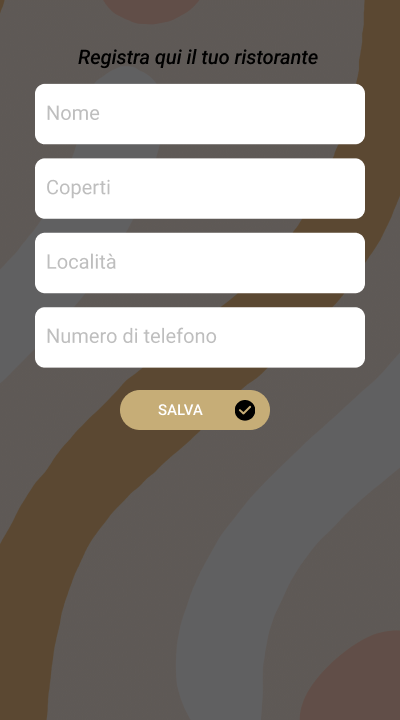
\includegraphics[scale=0.35]{assets/Mockup/Mockup_SaveResturant.png}
            \caption{\textbf{M05}: Schermata di registrazione di un nuovo ristorante}\label{fig:Mockup_AddResturant}
        \end{figure}
        \begin{flushleft}
            \textbf{ID} \ \Large{\textit{\textbf{M05}}}
        \end{flushleft}
        \textbf{Componenti}:

        \begin{center}
          \begin{tblr}{hlines = {0.9pt}, vlines = {0.9pt}, row{1} = {marroneApp!60}, colspec = {X[c]X[c]X[c]}, width = \textwidth}
            \textbf{Tipo}  &   \textbf{Nome}  & \textbf{Funzione} \\
            Edit Text      &   NOME           & Permette di inserire il nome del nuovo ristorante\\
            Edit Text      &   LOCALITA'      & Permette di inserire la località del nuovo ristorante\\
            Edit Text      &   COPERTI        & Permette di inserire il n° dei coperti del nuovo ristorante\\
            Edit Text      &   NUMERO DI TELEFONO & Permette di inserire il contatto telefonico del ristorante \\
            Bottone        &   SALVA          & Quando cliccato salva il nuovo ristorante nel database e torna alla schermata \textit{\textbf{M04}} \\
          \end{tblr}
        \end{center}
        \newpage
        \subsubsection{Schermata di modifica di un ristorante}
        \begin{figure}[H]
            \centering
            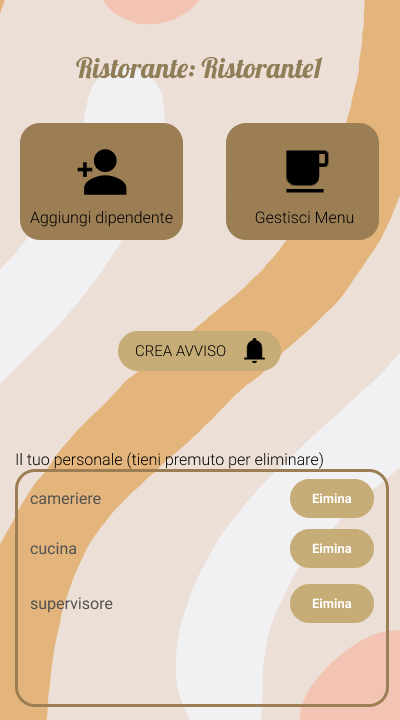
\includegraphics[scale=0.5]{assets/Mockup/Mockup_ResturantDash.png}
            \caption{\textbf{M06}: Schermata di modifica di un ristorante}\label{fig:Mockup_ResturantManager}
        \end{figure}
        \begin{flushleft}
            \textbf{ID} \ \Large{\textit{\textbf{M06}}}
        \end{flushleft}

        \textbf{Componenti}:

          \begin{center}
            \begin{tblr}{hlines = {0.9pt}, vlines = {0.9pt}, row{1} = {marroneApp!60}, colspec = {X[c]X[c]X[c]}, width = \textwidth}
              \textbf{Tipo}  &   \textbf{Nome}  & \textbf{Funzione} \\
              \textbf{Tipo}   &   \textbf{Nome}   &   \textbf{Funzione} \\
              Bottone   &   AGGIUNGI DIPENDENTE &   Quando cliccato porta alla schermata \textit{\textbf{M07}}\\
              Bottone   &   GESTISCI MENU &   Quando cliccato porta alla schermata \textit{\textbf{M08}}\\
              ScrollView  & IL TUO PERSONALE  & Mostra il personale che lavora nel ristorante \\
              Bottone   &   CREA AVVISO   &   Quando cliccato mostra la schermata \textit{\textbf{M17}} \\  
            \end{tblr}
          \end{center}

        \newpage

        \subsubsection{Schermata di registrazione di un nuovo dipendente}
        \begin{figure}[H]
            \centering
            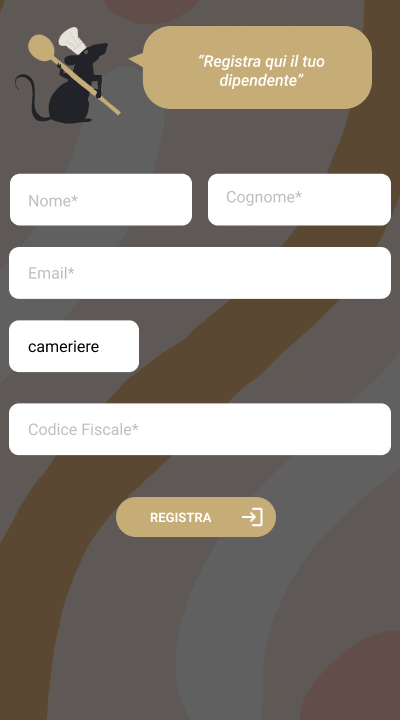
\includegraphics[scale=0.35]{assets/Mockup/Mockup_SaveWorker.png}
            \caption{\textbf{M07}: Schermata di registrazione di un nuovo dipendente}\label{fig:Mockup_SaveWaiter}
        \end{figure}
        \begin{flushleft}
            \textbf{ID} \ \Large{\textit{\textbf{M07}}}
        \end{flushleft}
        \textbf{Componenti}:

        \begin{center}
          \begin{tblr}{hlines = {0.9pt}, vlines = {0.9pt}, row{1} = {marroneApp!60}, colspec = {X[c]X[c]X[c]}, width = \textwidth}
            \textbf{Tipo}   &   \textbf{Nome}   &   \textbf{Funzione} \\
            Edit Text   &   NOME    &   Permette di inserire il nome del nuovo dipendente\\
            Edit Text   &   COGNOME   &   Permette di inserire il cognome del nuovo dipendente\\
            Edit Text   &   EMAIL   & Permette di inserire l'email del nuovo dipendente\\
            Edit Text   &   CODICE FISCALE    &   Permette di inserire il codice fiscale del nuovo dipendente \\
            Spinner &   {cameriere\\ (default)}    &   Permette di inserire il ruolo del nuovo dipendente \\
            Bottone &   REGISTRA    &   Quando cliccato, se tutti i dati sono corretti, riporta alla schermata \textit{\textbf{M04}} registrando il nuovo dipendente \\
          \end{tblr}
        \end{center}

        \newpage

        \subsubsection{Schermata di gestione del menù}
        \begin{figure}[H]
            \centering
            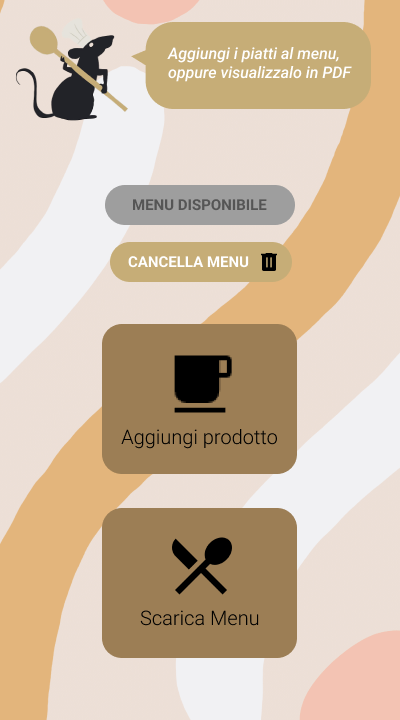
\includegraphics[scale=0.5]{assets/Mockup/Mockup_MenuManager.png}
            \caption{\textbf{M08}: Schermata di gestione del menù}\label{fig:Mockup_MenuManager}
        \end{figure}
        \begin{flushleft}
            \textbf{ID} \ \Large{\textit{\textbf{M08}}}
        \end{flushleft}
        \textbf{Componenti}:

        \begin{center}
          \begin{tblr}{hlines = {0.9pt}, vlines = {0.9pt}, row{1} = {marroneApp!60}, colspec = {X[c]X[c]X[c]}, width = \textwidth}
            \textbf{Tipo}   &   \textbf{Nome}   &   \textbf{Funzione} \\
            Bottone   &   AGGIUNGI PRODOTTO    &   Quando cliccato porta alla schermata \textit{\textbf{M18}}\\
            Edit Text   &   SCARICA MENU   &   Permette di generare il menù e salvarlo sul dispositivo in formato PDF\\
            Bottone   &   CREA MENU       &   Quando cliccato permette di creare un menu (se non è gia stato creato)
          \end{tblr}
        \end{center}

        \newpage

        \subsubsection{Schermata home per i supervisori}
          \begin{figure}[H]
              \centering
              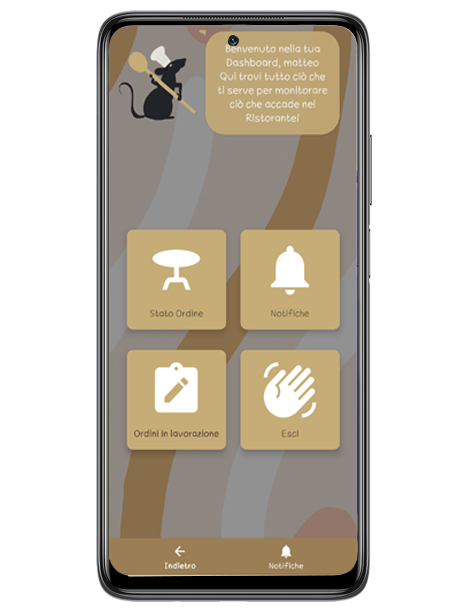
\includegraphics[scale=2.5]{assets/Mockup/Mockup_HypervisorDash.png}
              \caption*{\textbf{M09}: Schermata home dei supervisori}\label{fig:Mockup_HypervisorDash}
          \end{figure}

          \begin{flushleft}
              \textbf{ID}   \ \Large{\textit{\textbf{M09}}}
          \end{flushleft}

          \textbf{Componenti}:

          \begin{center}
              \begin{tblr}{hlines = {0.9pt}, vlines = {0.9pt}, row{1} = {marroneApp!60}, colspec = {X[c]X[c]X[c]}, width = \textwidth}
                \textbf{Tipo}   &   \textbf{Nome}   &   \textbf{Funzione} \\
                Bottone   &   STATO ORDINE    &   Quando cliccato porta alla schermata \textit{\textbf{M0bho}} \\
                Bottone   &   NOTIFICHE       &   Quando cliccato \\ %Inserire cosa fa
                Bottone   &   ORDINI IN LAVORAZIONE & \\ %Questo non l'ho capito
                Bottone   &   ESCI    &   Quando cliccato porta alla schermata \textit{\textbf{M10}} \\
                %TODO: Vedere la barra sotto come rappresentarla
              \end{tblr}
          \end{center}

        \newpage

        \subsubsection{Schermata di conferma di logout}
          \begin{figure}[H]
            \centering
            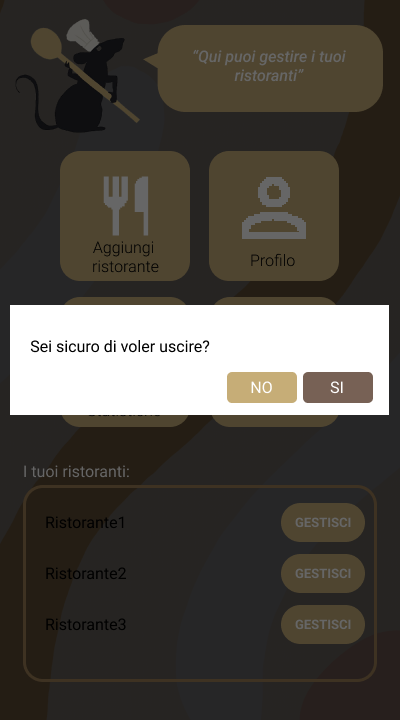
\includegraphics[scale=2]{assets/Mockup/Mockup_ExitDialog.png}
            \caption*{\textbf{M10}: Schermata di conferma logout}\label{fig:Mockup_ExitDialog}
          \end{figure}

          \begin{flushleft}
            \textbf{ID}   \ \Large{\textit{\textbf{M10}}}
          \end{flushleft}

          \textbf{Componenti}:

          \begin{center}
            \begin{tblr}{hlines = {0.9pt}, vlines = {0.9pt}, row{1} = {marroneApp!60}, colspec = {X[c]X[c]X[c]}, width = \textwidth}
              \textbf{Tipo}   &   \textbf{Nome}   &   \textbf{Funzione} \\
              Bottone         &   SI      &   Quando cliccato porta alla schermata \textit{\textbf{M02}} \\
              Bottone         &   NO      &   Quando cliccato resta nella schermata corrente \\
            \end{tblr}
          \end{center}
        
        \newpage

        \subsubsection{Schermata home per i camerieri}
          \begin{figure}[H]
            \centering
            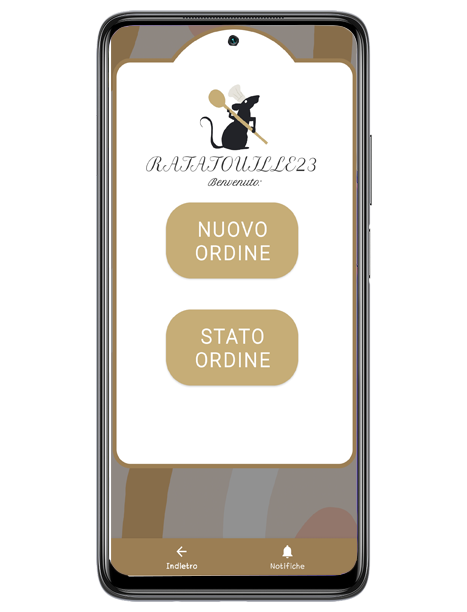
\includegraphics[scale=2]{assets/Mockup/Mockup_WaiterDash.png}
            \caption*{\textbf{M11}: Schermata home per i camerieri}\label{fig:Mockup_WaiterDash}
          \end{figure}

          \begin{flushleft}
            \textbf{ID}   \ \Large{\textit{\textbf{M11}}}
          \end{flushleft}

          \textbf{Componenti}:
          
          \begin{center}
            \begin{tblr}{hlines = {0.9pt}, vlines = {0.9pt}, row{1} = {marroneApp!60}, colspec = {X[c]X[c]X[c]}, width = \textwidth}
              \textbf{Tipo}   &   \textbf{Nome}   &   \textbf{Funzione} \\
              Bottone     &   NUOVO ORDINE    &   Quando cliccato porta alla schermata \textit{\textbf{M19}} \\
              Bottone     &   STATO ORDINE    &   Quando cliccato porta alla schermata \textit{\textbf{M0bho}} \\
              % TODO: Vedere la barra sotto come rappresentarla
            \end{tblr}
          \end{center}

        \newpage

        \subsubsection{Schermata home per la cucina}
  
            \begin{flushleft}
              \textbf{ID}   \ \Large{\textit{\textbf{M12}}}
            \end{flushleft}
  
            \textbf{Componenti}:
            
            \begin{center}
              \begin{tblr}{hlines = {0.9pt}, vlines = {0.9pt}, row{1} = {marroneApp!60}, colspec = {X[c]X[c]X[c]}, width = \textwidth}
                \textbf{Tipo}   &   \textbf{Nome}   &   \textbf{Funzione} \\
  
              \end{tblr}
            \end{center}

            \newpage

            \subsubsection{Schermata di visualizzazione del profilo}
              \begin{figure}[H]
                \centering
                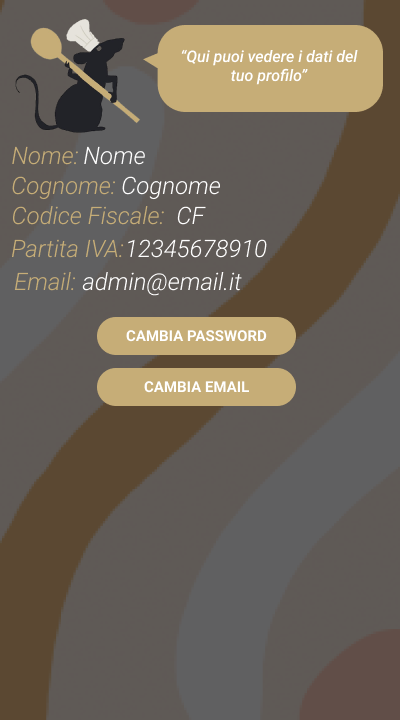
\includegraphics[scale=2.5]{assets/Mockup/Mockup_Profile.png}
                \caption*{\textbf{M13}: Schermata visualizzazione profilo}\label{fig:Mockup_Profile}
              \end{figure}
    
              \begin{flushleft}
                \textbf{ID}   \ \Large{\textit{\textbf{M13}}}
              \end{flushleft}
    
              \textbf{Componenti}:
              
              \begin{center}
                \begin{tblr}{hlines = {0.9pt}, vlines = {0.9pt}, row{1} = {marroneApp!60}, colspec = {X[c]X[c]X[c]}, width = \textwidth}
                  \textbf{Tipo}   &   \textbf{Nome}   &   \textbf{Funzione} \\
                  Bottone     &   CAMBIA PASSWORD   &   Quando cliccato mostra la schermata \textit{\textbf{M14}}  \\
                  Bottone     &   CAMBIA EMAIL   &   Quando cliccato mostra la schermata \textit{\textbf{M15}}  \\    
                \end{tblr}
              \end{center}

              \newpage

              \subsubsection{Schermata di cambio password per gli admin}
                \begin{figure}[H]
                  \centering
                  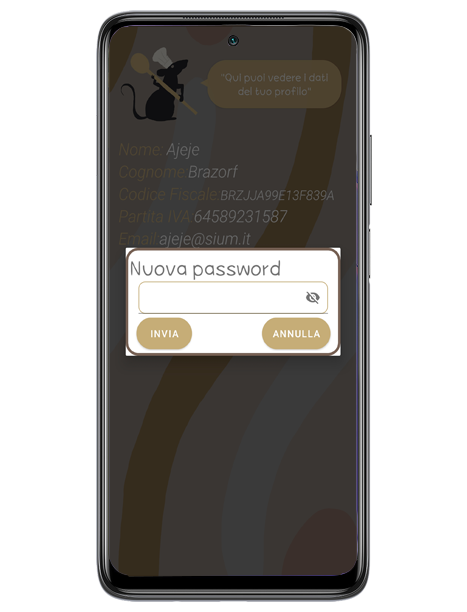
\includegraphics[scale=2.5]{assets/Mockup/Mockup_AdminChangePass.png}
                  \caption*{\textbf{M14}: Schermata cambio password admin}\label{fig:Mockup_AdminChangePass}
                \end{figure}
      
                \begin{flushleft}
                  \textbf{ID}   \ \Large{\textit{\textbf{M14}}}
                \end{flushleft}
      
                \textbf{Componenti}:
                
                \begin{center}
                  \begin{tblr}{hlines = {0.9pt}, vlines = {0.9pt}, row{1} = {marroneApp!60}, colspec = {X[c]X[c]X[c]}, width = \textwidth}
                    \textbf{Tipo}   &   \textbf{Nome}   &   \textbf{Funzione} \\
                    Edit Text     &   NUOVA PASSWORD    &   Permette di inserire la nuova password per l'account dell'admin   \\
                    Bottone     &   ANNULLA   &   Quando cliccato torna alla schermata \textit{\textbf{M13}} senza effettuare modifiche  \\
                    Bottone     &   INVIA   &   Quando cliccato torna alla schermata \textit{\textbf{M13}} modificando la password dell'account  \\
                  \end{tblr}
                \end{center}

                \newpage

                \subsubsection{Schermata di cambio email per gli admin}
                  \begin{figure}[H]
                    \centering
                    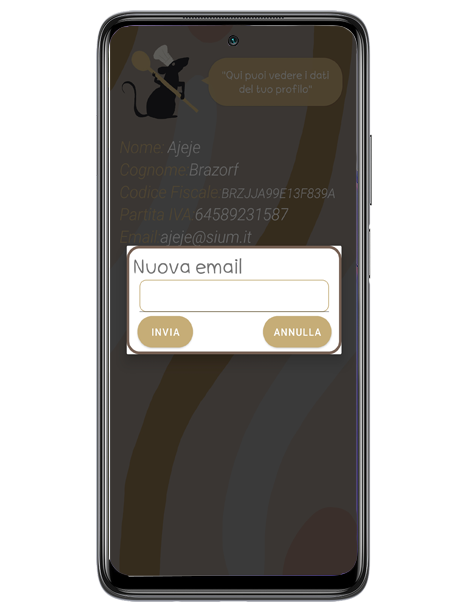
\includegraphics[scale=2.5]{assets/Mockup/Mockup_AdminChangeMail.png}
                    \caption*{\textbf{M15}: Schermata cambio email admin}\label{fig:Mockup_AdminChangeMail}
                  \end{figure}
        
                  \begin{flushleft}
                    \textbf{ID}   \ \Large{\textit{\textbf{M15}}}
                  \end{flushleft}
        
                  \textbf{Componenti}:
                  
                  \begin{center}
                    \begin{tblr}{hlines = {0.9pt}, vlines = {0.9pt}, row{1} = {marroneApp!60}, colspec = {X[c]X[c]X[c]}, width = \textwidth}
                      \textbf{Tipo}   &   \textbf{Nome}   &   \textbf{Funzione} \\
                      Edit Text   &   NUOVA EMAIL   &   Permette di inserire la nuova email per l'account dell'admin  \\
                      Bottone     &   ANNULLA   &   Quando cliccato torna alla schermata \textit{\textbf{M13}} senza effettuare modifiche  \\
                      Bottone     &   INVIA   &   Quando cliccato torna alla schermata \textit{\textbf{M13}} modificando l'email dell'account  \\
                    \end{tblr}
                  \end{center}

                \newpage

                \subsubsection{Schermata di cambio password per i dipendenti al primo accesso}
                    \begin{figure}[H]
                      \centering
                      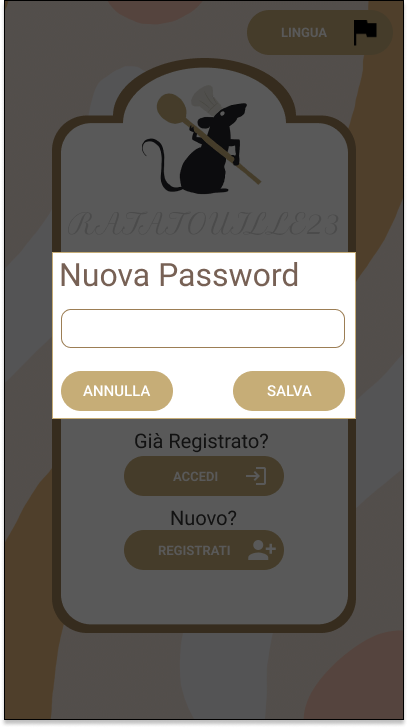
\includegraphics[scale=2]{assets/Mockup/Mockup_WorkerChangePass.png}
                      \caption*{\textbf{M16}: Schermata cambio password dipendenti}\label{fig:Mockup_WorkerChangePass}
                    \end{figure}
          
                    \begin{flushleft}
                      \textbf{ID}   \ \Large{\textit{\textbf{M16}}}
                    \end{flushleft}
          
                    \textbf{Componenti}:
                    
                    \begin{center}
                      \begin{tblr}{hlines = {0.9pt}, vlines = {0.9pt}, row{1} = {marroneApp!60}, colspec = {X[c]X[c]X[c]}, width = \textwidth}
                        \textbf{Tipo}   &   \textbf{Nome}   &   \textbf{Funzione} \\
                        Edit Text   &   NUOVA PASSWORD   &   Permette di inserire la nuova password per l'account del dipendente  \\
                        Bottone     &   ANNULLA   &   Quando cliccato torna alla schermata \textit{\textbf{M02}} senza effettuare modifiche  \\
                        Bottone     &   INVIA   &   Quando cliccato porta alla schermata \textit{\textbf{M09}} se è supervisore, \textit{\textbf{M11}} se è cameriere, \textit{\textbf{M12}} se è un account di cucina, modificando l'email dell'account  \\
                      \end{tblr}
                    \end{center}

                  \newpage

                  \subsubsection{Schermata di creazione degli avvisi}
                      \begin{figure}[H]
                        \centering
                        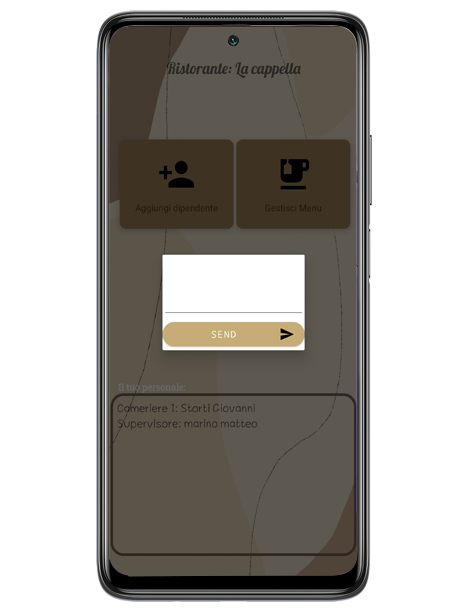
\includegraphics[scale=2.5]{assets/Mockup/Mockup_SaveAdv.png}
                        \caption*{\textbf{M17}: Schermata creazione avvisi}\label{fig:Mockup_SaveAdv}
                      \end{figure}
            
                      \begin{flushleft}
                        \textbf{ID}   \ \Large{\textit{\textbf{M17}}}
                      \end{flushleft}
            
                      \textbf{Componenti}:

                      \begin{center}
                        \begin{tblr}{hlines = {0.9pt}, vlines = {0.9pt}, row{1} = {marroneApp!60}, colspec = {X[c]X[c]X[c]}, width = \textwidth}
                          \textbf{Tipo}   &   \textbf{Nome}   &   \textbf{Funzione} \\
                          Edit Text     &   AVVISO    &   Permette di inserire il testo dell'avviso \\
                          Bottone       &   SEND      &   Quando cliccato torna alla schermata \textit{\textbf{M06}} inviando l'avviso \\
                        \end{tblr}
                      \end{center}

                    \newpage

                    \subsubsection{Schermata di aggiunta piatti al menù}
                        \begin{figure}[H]
                          \centering
                          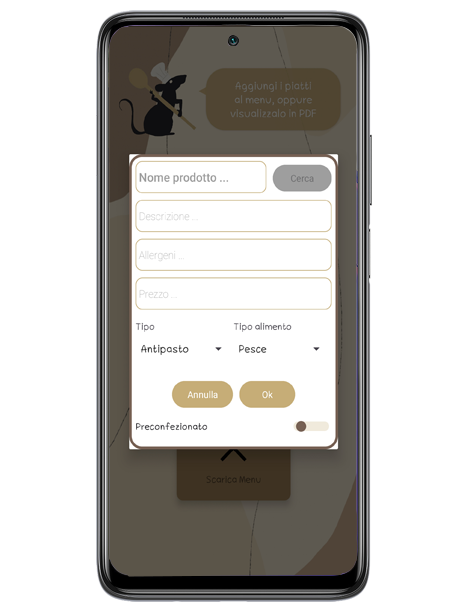
\includegraphics[scale=2]{assets/Mockup/Mockup_AddPlate.png}
                          \caption*{\textbf{M18}: Schermata aggiunta piatti al menù}\label{fig:Mockup_AddPlate}
                        \end{figure}
              
                        \begin{flushleft}
                          \textbf{ID}   \ \Large{\textit{\textbf{M18}}}
                        \end{flushleft}
              
                        \textbf{Componenti}:
                        
                        \begin{center}
                          \begin{longtblr}{hlines = {0.9pt}, vlines = {0.9pt}, row{1} = {marroneApp!60}, colspec = {X[c]X[c]X[c]}, width = \textwidth, rowhead=1}
                            \textbf{Tipo}   &   \textbf{Nome}   &   \textbf{Funzione} \\
                            EditText        &   NOME PRODOTTO   &   Permette di inserire il titolo del prodotto da inserire \\
                            EditText        &   DESCRIZIONE     &   Permette di inserire la descrizione del prodotto da Inserire  \\
                            EditText        &   ALLERGENI       &   Permette di inserire gli allergeni contenuti nel prodotto \\
                            EditText        &   PREZZO          &   Permette di inserire il prezzo del prodotto \\
                            Spinner         &   TIPO            &   Permette di inserire il tipo di portata (antipasto, primo, ...) \\
                            Spinner         &   TIPO DI ALIMENTO &  Permette di inserire il tipo di alimento (carne, pesce, ...)  \\
                            Bottone         &   CERCA           &   Quando cliccato, ricerca il prodotto scritto nel database di OpenFoodFacts  \\
                            Bottone         &   OK              &   Quando cliccato, ritorna alla schermata \textit{\textbf{M08}} salvando nel menu il prodotto \\
                            Bottone         &   ANNULLA         &   Quando cliccate, ritorna alla schermata \textit{\textbf{M08}} senza salvare il prodotto \\  
                            Selettore       &   PRECONFEZIONATO &   Se selezionato, indica che l'oggetto è di tipo preconfezionato(bibita, ...) \\
                          \end{longtblr}
                        \end{center}

                      \newpage

                    \subsubsection{Schermata di aggiunta ordini}
                          \begin{figure}[H]
                            \centering
                            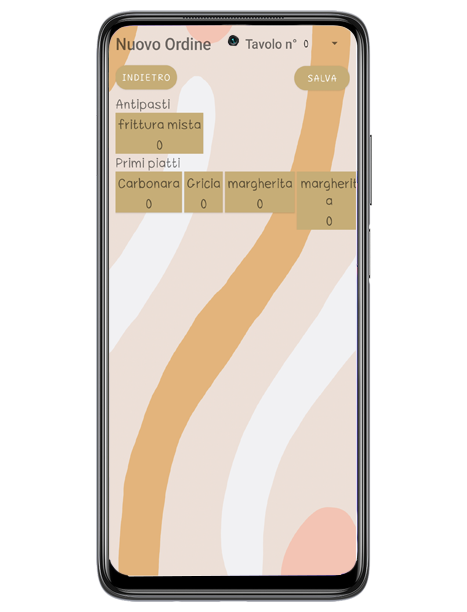
\includegraphics[scale=2]{assets/Mockup/Mockup_AddOrder.png}
                            \caption*{\textbf{M19}: Schermata aggiunta ordini}\label{fig:Mockup_WaiterDash}
                          \end{figure}
                
                          \begin{flushleft}
                            \textbf{ID}   \ \Large{\textit{\textbf{M19}}}
                          \end{flushleft}
                
                          \textbf{Componenti}:
                          
                          \begin{center}
                            \begin{tblr}{hlines = {0.9pt}, vlines = {0.9pt}, row{1} = {marroneApp!60}, colspec = {X[c]X[c]X[c]}, width = \textwidth}
                              \textbf{Tipo}   &   \textbf{Nome}   &   \textbf{Funzione} \\
                              ScrollView      &   PIATTI    &   Visualizza la lista dei piatti del menù del ristorante, dove ogni piatto si può cliccare per aggiungerlo all'ordine \\
                              Bottone         &   SALVA     &   Quando cliccato porta alla schermata \textit{\textbf{M11}} inviando l'ordine \\
                              Bottone         &   INDIETRO  &   Quando cliccato porta alla schermata \textit{\textbf{M11}} senza effettuare nessuna azione \\
                            \end{tblr}
                          \end{center}
    \subsection{Valutazione dell'usabilità}

    \begin{flushleft}
       Per la valutazione dell'usabilità del nostro applicativo a priori, cioè prima della fase di sviluppo vera a propria,
       abbiamo deciso di imporci come linee guida le euristiche di Nielsen.
       Ne sono 10, ma vorremmo richiamare l'attenzione su alcune di esse nello specifico:
        \begin{itemize}
            \item \textit{Visibilità dello stato del sistema.} Il sistema presentava una discreta mancanza di feedback, che prevediamo di colmare con elementi quali Dialog, Toast, AlertDialog e SnackBar.
            \item \textit{Prevenzione degli errori.} Il sistema reagisce in maniera controllata e predeterminata alle situazioni di errori che gli utenti possono causare. Nulla è lasciato al caso, ed è, nelle build provate dal team, gestita qualsiasi azione eseguibile dagli utenti.
            \item \textit{Riconoscere piuttosto che ricordare.} La nostra app è dotata di sezioni ben distinte, interfacce dinamiche a seconda del tipo di utente che le usa, e icone e testi ecplicativi dell'azione che si va a intrapendere.
            \item \textit{Guida e documentazione.} E' presente un simpatico topolino (che richiama il logo dell'app) che consiglia tramite vignette e piccoli dialoghi le azioni che si possono intraprendere. Inoltre ci sono piccole note come campi obbligatori ecc.
        \end{itemize}
    \end{flushleft}

    \begin{figure}[H]
        \centering
        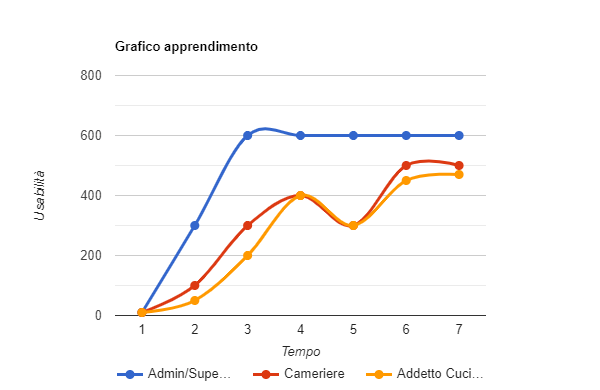
\includegraphics[scale=0.6]{assets/immagini varie/grafico usabilita.png}
        \caption{\textbf{Grafico}: Usabilità}\label{fig:Usabilità_graph}
    \end{figure}
\end{document}